\documentclass[11pt]{article}
\listfiles
\usepackage[letterpaper,margin=0.86in,headheight=15pt]{geometry}
\usepackage[T1]{fontenc}
\usepackage[utf8]{inputenc}
\usepackage{lmodern,microtype,amsmath,amssymb,booktabs,array,tabularx,longtable,graphicx,xcolor}
\usepackage[round,authoryear]{natbib}
\usepackage{enumitem,fancyhdr,titlesec,tcolorbox,caption,float,hyperref,needspace}
\DisableLigatures{encoding=*,family=lmtt}
\clubpenalty=10000
\widowpenalty=10000
\displaywidowpenalty=10000
\pretocmd{\section}{\Needspace{7\baselineskip}}{}{}
\pretocmd{\subsection}{\Needspace{5\baselineskip}}{}{}
\definecolor{nova}{HTML}{4C208A}
\definecolor{ink}{HTML}{181329}
\definecolor{mint}{HTML}{1E7466}
\definecolor{light}{HTML}{F3F0F9}
\definecolor{gold}{HTML}{A87521}
\hypersetup{colorlinks=true,linkcolor=nova,citecolor=nova,urlcolor=mint,pdftitle={Nova-Seeds: The Value That Survives Abundance},pdfauthor={MONTREAL.AI},pdfsubject={A reproducible calibration-aware allocation and copying experiment},pdfkeywords={appropriability, calibration, nonrival knowledge, verification, NovaSeed}}
\urlstyle{same}
\setlength{\parindent}{0pt}\setlength{\parskip}{0.5em}
\setlist{nosep,leftmargin=1.4em,topsep=4pt}
\titleformat{\section}{\Large\bfseries\color{nova}}{\thesection}{0.65em}{}
\titleformat{\subsection}{\large\bfseries\color{ink}}{\thesubsection}{0.65em}{}
\titlespacing*{\section}{0pt}{1.2em}{0.4em}
\titlespacing*{\subsection}{0pt}{0.8em}{0.25em}
\pagestyle{fancy}\fancyhf{}
\fancyhead[L]{\footnotesize\color{nova}NOVA-SEEDS / RESEARCH EDITION 1}
\fancyhead[R]{\footnotesize MONTREAL.AI}
\fancyfoot[L]{\scriptsize Synthetic instrument; measured computation; bounded claims}
\fancyfoot[R]{\thepage}
\renewcommand{\headrulewidth}{0.3pt}
\captionsetup{font=small,labelfont={bf,color=nova},skip=7pt}
\newcommand{\code}[1]{\texttt{\small #1}}
\newcommand{\Alpha}{\textsc{Alpha}}
\newcommand{\TI}{TI$\infty$}
\newcommand{\Om}{SUCCESSOR $\Omega$}
\newcommand{\scope}[1]{\begin{tcolorbox}[colback=light,colframe=nova!35,boxrule=0.5pt,arc=1.5mm,left=2mm,right=2mm,top=1mm,bottom=1mm]#1\end{tcolorbox}}
% Generated only from frozen analysis and separately labelled controls.
\newcommand{\HeadlineResult}{%
Shared calibration increases ordinary useful output by 37.3\%. The complete copy matches every mission. Conventional scheduling also obtains the benefit; under drift, fresh recalibration wins. What survives is a reusable capability, with no demonstrated exclusive output premium.
}

\newcommand{\AbstractResults}{%
Ordinary useful output rises from 23.81 to 32.69 synthetic units per mission: 37.3\% (paired 95\% interval 34.9--39.4\%). The complete clone matches all 3,072 plans and outcomes; an independently written expert matches the stationary-model optimum. The greedy competitor ties ordinary output with lower measured computing cost. Hidden drift reverses the baseline benefit, and delayed diagnostics let the adaptive competitor improve the next decision.
}

\newcommand{\MainResults}{%
The campaign completed all 3,072 worlds and 21,504 method records, with 0 method noncompletions. Ordinary mean useful output is 32.69 for the verified artifact and 23.81 for the conservative baseline. The paired difference is 8.88 units (95\% cluster-bootstrap interval 8.22--9.56), or 37.3\% (34.9--39.4\%). This exceeds the predeclared 5\% practical margin against that restriction.

There are zero complete-copy plan/outcome mismatches and zero independent-expert stationary-model objective mismatches. Disclosed and verified native planning yield the same productive outcomes; the extra evidence machinery is not awarded utility. The conventional greedy policy also ties ordinary useful output. These comparisons defeat an exclusive-performance interpretation of the primary improvement.

Doubled capacity, one-tick validity and zero-duration calibration eliminate the ordinary restriction's output gap. The result depends on the actual bottleneck: removing or changing that bottleneck removes the measured advantage over the ablation.
}

\newcommand{\ResultsTable}{%
\begin{table}[H]\small\renewcommand{\arraystretch}{1.13}
\begin{tabularx}{\textwidth}{@{}Xrrrr@{}}\toprule
Condition & Conservative & Verified$^{*}$ & Greedy & Adaptive\\\midrule
Ordinary & 23.81 & 32.69 & 32.69 & 32.69\\
Doubled capacity & 39.47 & 39.47 & 39.47 & 39.47\\
Short validity & 23.81 & 23.81 & 23.81 & 23.81\\
Measurement drift & 23.81 & 11.12 & 13.12 & 22.76\\
Demand drift & 24.08 & 33.17 & 33.17 & 33.17\\
Slot failures & 18.72 & 25.75 & 25.79 & 25.75\\
Zero-duration calibration & 32.69 & 32.69 & 32.69 & 32.69\\
Repeated inspection & 23.81 & 32.69 & 32.69 & 32.69\\
\bottomrule\end{tabularx}
\caption{Mean true useful output in synthetic units. Each entry averages 384 missions in 32 seed clusters. $^{*}$The complete clone, disclosed planner and stationary exact expert have the same mean output; raw exact predicates and all method-specific intervals remain in the machine-readable analysis. These policies are counterfactual alternatives, not additive production.}
\end{table}
}

\newcommand{\DriftResults}{%
Under measurement drift, the verified artifact earns 11.12 units per mission versus 23.81 for conservative recalibration and 22.76 for the adaptive expert. The verified-minus-adaptive difference is -11.63 units (descriptive interval -12.35 to -10.91). The native proof remains correct about its stationary model while two later-slot measurements are wrong. More complete internal verification does not make that model physically true.

The adaptive expert receives no earlier private warning. At the first epoch it has the same stationary prior; subsequent recovery uses the prior epoch's public delayed bias profile. The conservative policy has the highest full-horizon output by paying for fresh calibration. The adaptive expert ties it in epochs two through twelve but cannot recover its first-epoch loss. This unfavorable result identifies the assumption that fails, rather than treating lost output as an outlier.

The greedy comparator earns 13.12 units without observing future drift: it places a high-value sample first, before the hidden shift. For seed 101's first epoch, job weights are 7, 11, 13 and 13. The native and stationary exact plans place weight 11 in the surviving first measurement slot; greedy places weight 13 there. Both optimize the nominal stationary objective. Different optimal-model tie breaking can therefore matter after the model fails. Under random slot failures, greedy's slightly higher sample mean is a descriptive fluctuation, not an established reliability advantage.
}

\newcommand{\ComputeResults}{%
In ordinary operation, the verified native service uses 70.738 ms of attributed CPU per mission, compared with 4.861 ms for the exact expert and 2.731 ms for the signed greedy service. All three have the same ordinary useful output. These descriptive timings include the common external evaluator and receipt-service setup where present; they do not include unknown authoring labor.

Copying 23 files (204,508 bytes) took 2.003 ms on the prepared host. The copied worker's startup/import took 57.900 ms; its evidence-module import took 2.753 ms. Fresh complete execution then matched every mission. These are measured software operations, not a measured time for an outside organization to acquire equipment, understand the work, or enter a market.
}

\newcommand{\CostTable}{%
\begin{table}[H]\small\renewcommand{\arraystretch}{1.13}
\begin{tabularx}{\textwidth}{@{}Xrrrr@{}}\toprule
Ordinary policy & CPU, ms & Calibrations & Samples & Receipt, bytes\\\midrule
Conservative & 2.369 & 2.0 & 2.0 & 0\\
Greedy & 2.731 & 1.0 & 3.0 & 881\\
Disclosed & 37.461 & 1.0 & 3.0 & 0\\
Verified & 70.738 & 1.0 & 3.0 & 887\\
Complete clone & 73.854 & 1.0 & 3.0 & 884\\
Exact expert & 4.861 & 1.0 & 3.0 & 881\\
Adaptive expert & 4.802 & 1.0 & 3.0 & 890\\
\bottomrule\end{tabularx}
\caption{Per-mission means. Each policy has a four-tick contested horizon plus four auxiliary diagnostic acquisitions outside it. Receipt bytes omit native completion/model exports, retained separately. CPU is measured; acquisition counts are simulated.}
\end{table}
The confirmation's measured process total is 733.416 CPU seconds (63.655 parent and 669.760 across both native workers), over 755.168 wall seconds. The runner's recorded raw/ledger/completion storage is 14,990,356 bytes. These totals cover all tested alternatives and shared harness work; they are not the resource bill of one deployed policy. Each policy's counterfactual horizon contains 12,288 auxiliary diagnostic acquisitions. It would be incorrect to present the sum over seven policies as physical laboratory production.
}

\newcommand{\AdditionalCosts}{%
\begin{table}[H]\small\renewcommand{\arraystretch}{1.1}
\begin{tabularx}{\textwidth}{@{}Xrr@{}}\toprule
Separately recorded execution & CPU seconds & Wall seconds\\\midrule
Confirmation campaign & 733.416 & 755.168\\
Independent replay/signatures/ledgers & 10.853 & 10.448\\
48 retained native completions & 3.313 & 2.946\\
Closed-form objective audit & 1.409 & 1.410\\
Frozen statistical analysis & 8.943 & 8.148\\
Local EVM and registry demonstration & 2.085 & 2.220\\
Published dispatcher graph & 3.020 & 3.185\\
Separate Node development cases & 0.676 & 0.488\\
\bottomrule\end{tabularx}
\caption{Additional verification and mechanism costs are visible. Per-method CPU is already inside the campaign total and is not added again. Wall durations can overlap and are not summed as total elapsed time. Each lane retains its exact timer boundaries.}
\end{table}
The listed, distinct executions account for 763.716 CPU seconds. This is not a full research or deployment cost: dependency download/compilation, earlier development, native-route execution, authoring, layout and some process startup were not completely metered. The archive records these exclusions rather than assigning them a zero price.
}

\newcommand{\SensitivityResults}{%
For an explicitly hypothetical ordinary mission, assign value 1 per useful unit, price 1 per calibration and sample, and price 1 per CPU hour. The verified-minus-conservative modeled surplus is 8.87 arbitrary monetary units. Increasing only the sample price to 20 changes it to -10.13; alternatively, adding 10 units of otherwise omitted cost changes it to -1.13. These reversals show the dependence on unobserved resource valuations. No price in this calculation is a market quote or a measured willingness to pay. The archive retains all 240 condition/comparator/assumption combinations, including negative output differences and undefined positive-output break-even values.
}

\newcommand{\LifecycleResults}{%
The separately executed published-runtime bridge completes 16 actual pure callbacks across two eight-job graphs, all seven lifecycle families, 24 negative controls and 121 verified journal events. Fresh second-epoch world evidence, mission, institution, environment, release, authorization and reservations are required. Zero production grants are issued. The development-case Node work uses 487.965 ms wall and 676.216 ms CPU; the Python graph uses 3.185404 s wall and 3.020314 s CPU. Those are single-run measurements under concurrent host activity, with the documented timing exclusions.
}

\newcommand{\ClaimLedger}{%
\begingroup\small\begin{longtable}{@{}>{\raggedright\arraybackslash}p{0.29\textwidth}>{\raggedright\arraybackslash}p{0.30\textwidth}>{\raggedright\arraybackslash}p{0.35\textwidth}@{}}
\toprule Claim & Evidence/status & Cost and limit\\\midrule\endhead
Ordinary restriction removal helps & Paired primary comparison; supported in simulation & Extra sample replaces a calibration; supplied utility is not willingness to pay.\\
Exclusive output survives copying & Not supported: complete clone matches all missions & Actual copy and execution charged; human reconstruction time unknown.\\
Framework beats sufficient conventional planning & Not supported: ordinary output ties; native CPU is higher & Same signed service available to competitors; no scalability finding.\\
Proof guarantees real usefulness & Refuted by model-valid drift failures and signed falsehood & Failed work still consumes resources; no trusted hardware.\\
NFT improves instrument output & No measured increment in the binding-interface control & Local gas and registry CPU are different units; escrow not reproduced.\\
Confidentiality equals productive superiority & Not supported; AES-GCM control only & Equal authorized plaintext; public synthetic workloads are not secret.\\
All native integrations admit the new mission & Unqualified/unavailable & Existing supported mission and local published graph only; no live Fleet execution.\\
Full-cost profitability or permanent capture & Unknown; no observed customer revenue & Human, physical, liability and demand costs unmeasured.\\
\bottomrule\end{longtable}\endgroup
}

\newcommand{\FreezeIdentity}{%
Source inventory SHA-256:\par\noindent{\small\texttt{0011228ddfd4a2e822659a0286864211b6c8eb99b93a3e39b9ba2cd3a582d08a}}\par Protocol/source/analysis freeze SHA-256:\par\noindent{\small\texttt{caef3d4995f38326af143172a1f3153f2b5f3a796b269532830e3a3a6655193a}}\par Both were preserved and publicly registered in issue \#4850 before the confirmation. The final archive manifest records the canonical PDF digest and every payload member.
}

\begin{document}
\thispagestyle{empty}
{\color{nova}\small\bfseries MONTREAL.AI\quad /\quad TRANSFORMATIONAL INTELLIGENCE $\infty$}
\vspace{0.45cm}

{\fontsize{35}{38}\selectfont\bfseries\color{ink}NOVA-SEEDS}\par
\vspace{0.12cm}
{\fontsize{23}{27}\selectfont\bfseries The Value That\newline Survives Abundance\par}
\vspace{0.28cm}
{\large\color{nova}From Copyable Intelligence to Verified Productive Advantage}\par
\vspace{0.25cm}
{\small MONTREAL.AI\quad $\cdot$\quad Writer \#10\quad $\cdot$\quad Research edition v1}
\vspace{0.3cm}

{\small\itshape ``Nova-Seeds encode cosmic foresight, quietly locking away and igniting profound scarcity; invisible intelligence greater than markets reshapes economic destiny.''}\par
{\scriptsize\color{nova}A poetic provocation, not a scientific finding.}
\vspace{0.22cm}

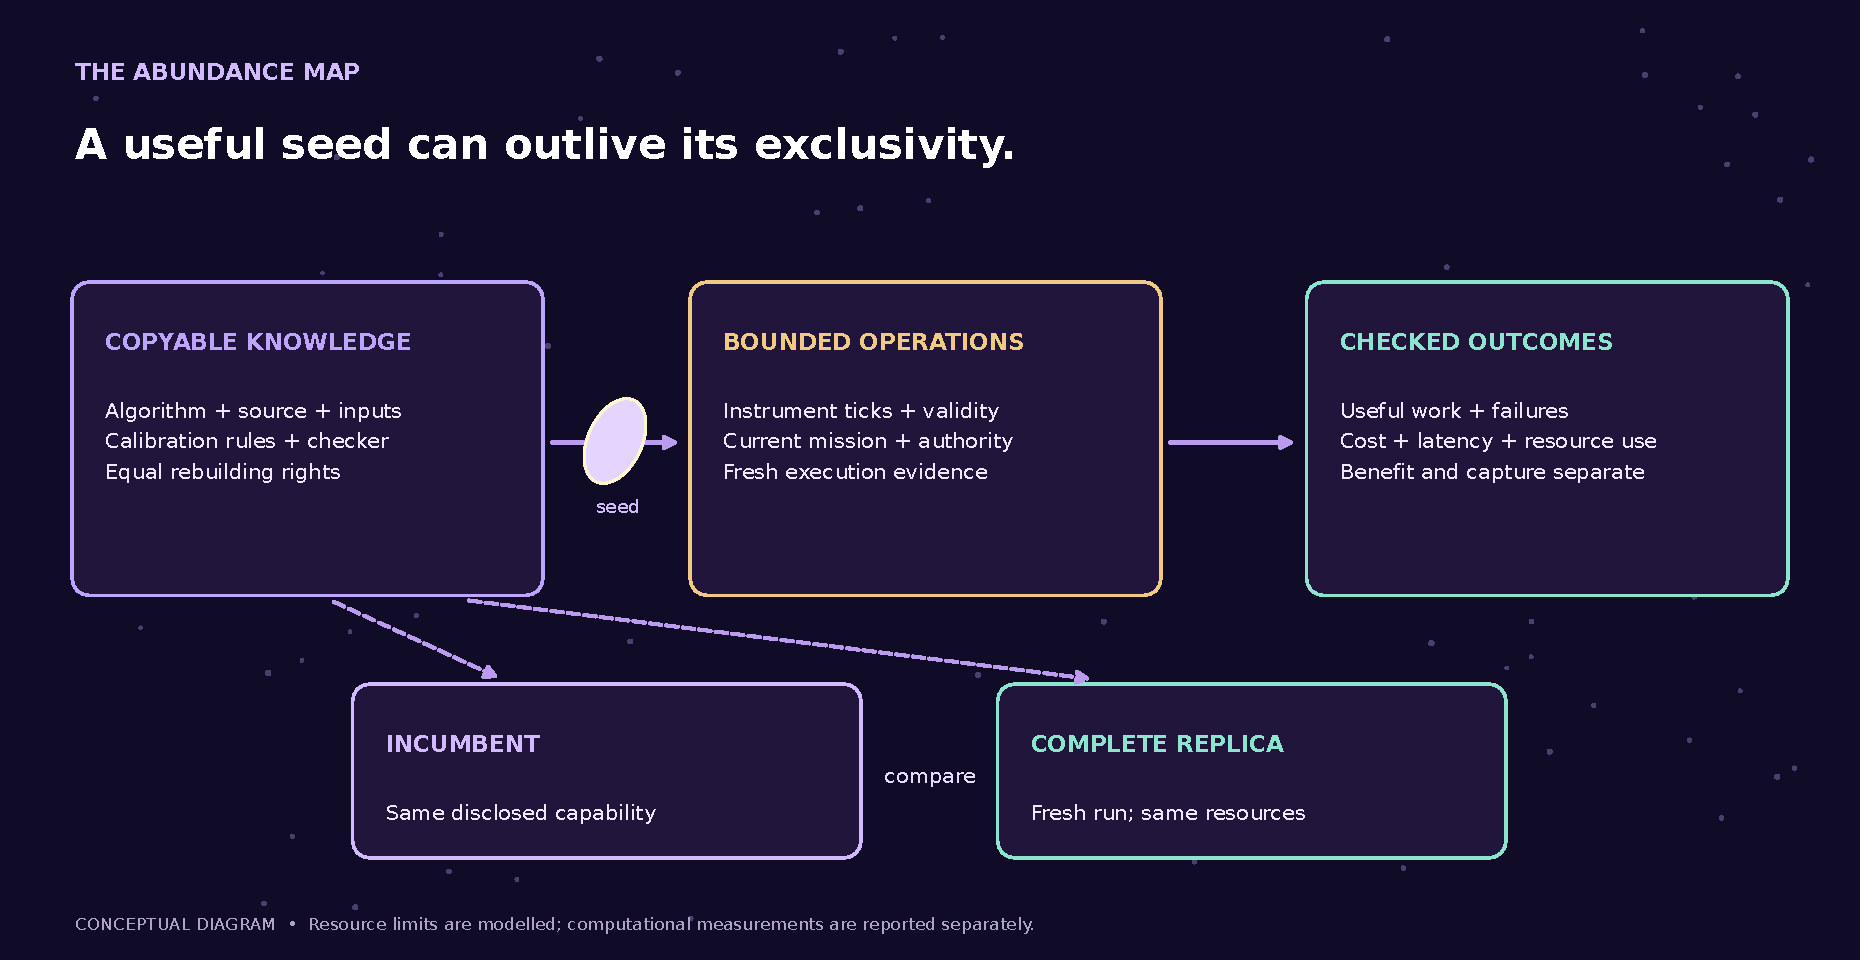
\includegraphics[width=\textwidth]{../figures/abundance-map.pdf}

\vspace{0.3cm}
\textbf{The question.} When an algorithm, its implementation and its inputs can be copied, what remains useful---and what remains exclusively valuable to its inventor?

\textbf{The experiment.} Construct a calibration-aware allocation service. Expose the complete system to a fresh replica and competent competitors. Check outcomes, resources, receipts, drift and a no-NFT alternative.

\textbf{The result.} \HeadlineResult

\vfill
{\footnotesize\color{nova}A useful seed can outlive its exclusivity.}\hfill{\footnotesize Versioned, reproducible, locally executed}
\clearpage

\begin{abstract}
Cheaply reproducible intelligence can expand productive possibilities without preserving its inventor's private advantage. We test that distinction in a deliberately tractable synthetic instrument. The constructed capability replaces mandatory recalibration before each occupied measurement tick with valid shared calibration, compiled into an existing finite optimizer and accompanied by independently checkable execution evidence. We predeclare eight conditions, 32 paired seeds and 12 epochs, comparing seven methods over 3,072 worlds and 21,504 method records. The implementation reuses pinned modules from Alpha, Jobs and Fleet; both existing currency-specific native routes are separately exercised on their actually supported mission. \AbstractResults\ A separate local-EVM lifecycle binds six-world pilot evidence to all five Ascension contracts; an off-chain signed registry preserves the studied productive result and evidence-binding functions without claiming equivalent escrow or public consensus. Every physical outcome is simulated, monetary demand and authoring cost remain unmeasured, and no commercial profitability is established. The contribution is an executable, source-bound test of productive value under copying, with negative results and trust boundaries retained.
\end{abstract}

\scope{\textbf{Reading key.} \textbf{Implemented} means code executed here. \textbf{Measured} refers to recorded computation, bytes or local-EVM gas. \textbf{Simulated} describes instrument state, job value, calibration and failures. \textbf{Assumed} marks economic prices and diagnostic access. \textbf{Unresolved} marks physical validation, external trust, real demand and full cost. None of these labels is interchangeable.}

\section{A three-minute journey}
The opening provocation is poetry. We turn it into a question to investigate. A seed is useful when another operator can grow a capability from it. The scientific question is whether any measured advantage remains when that operator has the same knowledge and rebuilding rights: what survives, who can capture it, for how long, and at what cost?

Imagine a small laboratory instrument with four available ticks. A calibration consumes one tick. Under a conservative procedure, the instrument calibrates, measures, calibrates again, and measures again. Two measurements fit. Under the declared stationary-bias model, a calibration remains valid for three ticks: calibrate once, then measure three times. The enabling intervention is a reusable allocation and evidence artifact that makes this less restrictive procedure explicit and checkable.

The first improvement is useful only relative to a stated alternative. A conventional scheduler can also reuse calibration. The complete source replica receives the same jobs, resource capacity, calibration rules and delayed diagnostics, then constructs fresh plans and signatures. It does not receive incumbent-only data, inherit an old mission's permission, or win by replaying another actor's receipt. An independently written enumerator and a simpler greedy scheduler test whether the native framework contributes anything beyond familiar scheduling.

Now change the world. The instrument's bias shifts after the first measurement. A schedule can remain valid under the supplied model while its corrected measurements become wrong. Its signature remains valid too. A competitor using the previous epoch's delayed quality report can schedule a fresh calibration and recover useful work. That recovery relies on an explicitly assumed auxiliary diagnostic channel, with four reference acquisitions counted separately per epoch.

Finally remove the NFT layer. The same results can be entered into a signed off-chain registry. If productive outcomes stay unchanged, the token layer has not demonstrated a productivity contribution in this experiment. Its implemented escrow and shared-state semantics may answer other institutional questions; those require their own threat models and evidence.

\textbf{What the reader should remember:} removing a needless operational restriction can create reusable public benefit. Copyability, model error and a cheaper adequate verifier can simultaneously eliminate a claim to exclusive advantage.

\section{What counts as value?}
\subsection{Separate properties before measuring them}
\begin{table}[H]\small\renewcommand{\arraystretch}{1.16}
\begin{tabularx}{\textwidth}{@{}p{0.22\textwidth}X@{}}\toprule
Concept & Operational meaning in this study\\\midrule
Physical scarcity & A finite simulated instrument horizon; no real apparatus was booked or measured.\\
Economic rivalry & Two simultaneous uses of the same occupied tick can conflict. A copied file does not create another tick.\\
Technical nonrivalry & The disclosed source and data can be used by multiple operators without consuming the original.\\
Artificial restriction & An admission rule, denied access or withheld key. Such a rule is not evidence of better productive performance.\\
Useful output & Job weight earned only by an attempted measurement that survives failure and error checks.\\
Productive advantage & A difference in useful output or resource cost relative to an equally equipped named alternative.\\
Private capture & Revenue actually received or explicitly modeled, with costs separately deducted. No customer proceeds are observed here.\\
Social benefit & Incremental useful outcomes minus valued resource costs; job weights are synthetic proxies, not measured welfare.\\\bottomrule
\end{tabularx}
\caption{Distinct questions with distinct evidence. Token balances and NFT prices are absent from the productive-output metric.}
\end{table}

For a policy $\pi$ in mission $m$, let $a_{jm}$ indicate an attempted job, $q_{jm}$ its true simulated quality/failure acceptance, and $v_{jm}$ its supplied utility weight. We measure
\begin{equation}
U_m(\pi)=\sum_j v_{jm}a_{jm}(\pi)q_{jm}(\pi),\qquad
\Delta U_m(\pi,b)=U_m(\pi)-U_m(b).
\end{equation}
The same external evaluator computes $q$ for every method. Missing signatures do not turn valid output into zero. Conversely, a valid signature does not turn failed output into useful work.

Define residual advantage against the tested equipped alternatives $\mathcal B$ as
\begin{equation}
A_m(\pi;\lambda)=U_m(\pi)-\lambda^\top C_m(\pi)
-\max_{b\in\mathcal B}\{U_m(b)-\lambda^\top C_m(b)\},
\end{equation}
where $C$ retains separate resource classes and $\lambda$ is a stated conversion vector. There is no universally valid exchange rate between a simulated acquisition, CPU time and user benefit. We report the vector first. A nonpositive $A$ is compatible with positive $\Delta U$ against a conservative baseline.

Private profit is a further quantity, $\Pi=R-C_{\rm operating}-C_{\rm construction}-C_{\rm opportunity}$. Unknown human effort, instrument cost and demand prevent a full-profit estimate. A modeled price is not revenue; revenue is not profit; a transfer between operators is not an additional social outcome. Each policy is a counterfactual use of the same resource budget. Summing all seven policy outputs would count the same offers repeatedly.

``Survives abundance'' therefore has three possible meanings: a useful capability still works after disclosure; a cost or service advantage remains against equipped rivals; or an operator captures a net return under stated market conditions. The experiment measures the first two within its finite model and leaves commercial capture conditional.

\section{Foundations and contribution}
Arrow distinguishes the usefulness of information from the difficulty of appropriating its returns \citep{arrow1962}. Romer distinguishes rivalry from excludability \citep{romer1990}. Teece explains why complementary assets and imitation conditions can determine who captures the returns from an innovation \citep{teece1986}. These are prior foundations, not laws discovered by Nova-Seeds. A finite instrument is a complement; simply naming it does not prove exclusivity, durability or profit.

Data are also nonrival, while ownership and access affect their use \citep{jonestonetti2020}. Data-enabled learning can produce different competitive effects depending on how learning accumulates and transfers \citep{hagiuwright2023}. Our matched test deliberately removes an incumbent-only data lead. It cannot establish that such leads never matter in real markets.

Calibration-aware scheduling is established work. \citet{bender2013} study calibration validity windows and give an optimal polynomial-time algorithm for a single-machine, unit-time case. Their calibration is instantaneous. Our small model includes a positive-duration calibration bottleneck, a different weighted-output objective, an explicitly misspecified drift condition, and executable receipt/copying tests. We make no new scheduling-complexity claim. The finite geometry is deliberately small enough for exhaustive independent comparison.

Proof-carrying code verifies specified program properties \citep{neculalee1996,necula1997}. Combining semantic reasoning with accountable authority is also established \citep{whitehead2004}. Our artifact carries executable model checks and authenticated statements; it is not a new cryptographic proof system or a formal proof of physical truth. Calibration intervals here are synthetic assumptions. NIST's guidance is application-specific, and traceability alone does not establish fitness for purpose \citep{nistinterval2026,nisttraceability2021}.

The project's \emph{Transformational Intelligence}, \emph{Invent the Economy}, and recovered \emph{Possibility Foundry} were read from pinned source. They motivate changing a formulation while preserving the purpose, separating productive outcomes from cash, and retaining strong counterexamples. The recovered Foundry's cheaper matched comparisons and $0/128$ narrow-line result are preserved as historical findings, not reused as our observations. Writer \#10 does not use Writer \#6's manuscript or results. Writers \#8 and \#9 concern macro capacity and foresight/timing respectively; their assigned directions are not treated as completed evidence for this study.

\textbf{Our contribution} is a reproducible operational experiment joining a constructed calibration capability, exact source-bound checks, complete copying, conventional rebuilding, drift adaptation, and registry substitution. Its result is the measured boundary between shared usefulness and private advantage. The novelty claimed is this implemented test and integration, not a new theory of information economics, scheduling law, or cryptographic primitive.

\section{The constructed capability}
\subsection{A four-tick instrument with explicit semantics}
Each mission offers four one-tick jobs. A job is rejected or assigned to measurement slot $1$, $2$ or $3$. Binary variables $c_0,c_1,c_2$ select calibration ticks. There are $2^3 4^4=2{,}048$ complete assignments. Normally, a calibration monopolizes its tick and a measurement tick holds one job. A job is model-valid if a preceding calibration exists and its age does not exceed that job's inclusive time-to-live. The capacity condition allows two samples per measurement tick; calibration still occupies the resource. In the cheap-calibration substitute, calibration duration is zero and same-tick calibration is permitted.

The constructed finite factor table excludes overlap, capacity violations and expired calibration. The native optimizer minimizes
\begin{equation}
L=100\sum_{j:\,s_j=0}v_j+\sum_{t=0}^{2}c_t.
\end{equation}
Integer utility is lexicographically primary: no three-calibration difference can outweigh one utility unit. This is an exact optimum of the supplied finite model. It is not an optimum over unknown future physical states or all conceivable scientific designs.

The enabling change is removal of the requirement to recalibrate before every occupied measurement tick. The conservative baseline retains that requirement; it is a deliberate capability ablation. The shared artifact and all competent rivals may exploit the same validity rule. Under doubled sample capacity, one immediate prior calibration can serve both simultaneous jobs, so ``per occupied tick'' is the accurate restriction.

\subsection{Execution and independent evaluation}
The simulated observation is $y_{jt}=x_j+b_t+\epsilon_{jt}$. Calibration at $c$ observes the exact bias $b_c$, and correction gives $\hat x_{jt}=y_{jt}-b_c$. A measurement is useful only if its slot does not fail and $|\hat x_{jt}-x_j|\leq0.25$. Noise lies in $[-0.05,0.05]$. The stationary planning model assumes $b_t=b_c$. The drift condition introduces an unobserved $+0.8$ shift at tick two. That violates the model without invalidating its internal calculation.

World generation, planning, model checking, and true-outcome replay are distinct steps. The independent evaluator imports no planner or table compiler. It directly enumerates assignments for the expert and replays measurements for every policy. Complete source and generation rules are disclosed. Realized future states are withheld equally until execution; mission identifiers do not encode condition or seed.

After each epoch, four auxiliary reference observations reveal the relative bias profile. Every method receives the identical delayed report in the next mission. The adaptive expert uses the previous profile and accepts predicted error only when the bias difference plus the known noise bound fits the tolerance. Other fixed policies intentionally ignore this report. This is a tested competitor capability, not a deprivation of incumbent rights. The ideal delayed diagnostic channel is separately counted and is not physical metrology evidence.

\subsection{Checkable evidence with fresh scope}
The allocation uses the actual Alpha finite optimizer and its completion inspector. The completion binds model, source, assignment, objective and counted work. Jobs supplies the existing Ed25519 implementation; Fleet supplies its outcome ledger. Each measured verified service has a fresh ephemeral signer and ledger, with a mission-specific fixture context. The copied native optimizer runs in a separate Node process; its copied receipt module runs in the parent process with a distinct key and ledger. This is software separation on one host, not organizational independence.

The complete clone receives identical current inputs and source, recomputes the schedule, checks it again, and produces its own receipt. It does not borrow the incumbent's key. The expert, adaptive expert and greedy competitor also receive the signed-record/ledger service, so reported verified-service costs do not compare a receipt-producing incumbent against an unverified competitor. The disclosed implementation omits extra external inspection and receipts; useful output remains evaluated identically. Native optimizer work and equivalent external service checks are itemized.

Fresh scoped fixture leases, purpose, time and mission checks establish only the local permission exercised. A predecessor's governance or evidence does not authorize a successor. The public archive retains public keys and signatures; no private signing or encryption key is persisted.

\section{Predeclared experiment}
The initial protocol and compiled checkpoint were saved privately, reopened and hash-verified before confirmation. Development used only the allowed seed range 1--8 and hand-written analytic examples. A development run encountered disk exhaustion and remains labelled incomplete; its raw records were losslessly compressed with original hashes. Streaming gzip was introduced before the final source freeze. A fresh six-world smoke campaign and focused checks qualified the revised serialization. No holdout seed was opened to repair the implementation or choose a favorable result.

The final protocol fixes 32 seeds, 12 epochs and eight conditions, yielding 3,072 matched worlds. Seven methods yield 21,504 method records. Every method receives the same current mission and previous diagnostic report. Invocation order rotates; a copied source tree and separate worker execute the complete native replica. The exact and adaptive experts are separately implemented direct enumerators; the simple greedy comparator is intentionally sufficient when the model permits it.

\begin{table}[H]\small\renewcommand{\arraystretch}{1.13}
\begin{tabularx}{\textwidth}{@{}p{0.27\textwidth}X@{}}\toprule
Method & Comparison being tested\\\midrule
Conservative idea operationalization & Best allocation while recalibrating before every occupied sample tick; capability-removal baseline.\\
Disclosed implementation & The same native shared-calibration plan; no extra external receipt inspection or signed ledger service.\\
Verified artifact & Native plan plus complete external inspection and scoped signed evidence.\\
Complete clone & Copied native/evidence source, fresh execution, separate ephemeral key and ledger, equivalent rights and inputs.\\
Independent exact expert & Separately authored exhaustive optimum for the public stationary planning model; signed replay evidence.\\
Conventional greedy & Value-first calibration reuse; independently replayed outcomes and signed evidence.\\
Adaptive expert & Exhaustive search using the previous epoch's delayed bias profile; signed replay evidence.\\\bottomrule
\end{tabularx}
\caption{The conservative baseline isolates the enabling restriction. The complete clone and conventional experts test whether that benefit is exclusively attributable to the artifact.}
\end{table}

The conditions are ordinary operation, doubled sample capacity, one-tick calibration validity, hidden measurement drift, public demand-weight drift after six epochs, shared stochastic slot failures, zero-duration calibration, and eight repeated evidence inspections. The first epoch has no prior diagnostic report. An instrument slot failure and an invalid measurement both consume resources. Every method's true synthetic output is scored identically.

The one primary contrast is the ordinary-condition useful-output improvement of the verified artifact over the conservative baseline, with a predeclared practical margin of 5\%. The independent unit is the seed: twelve epochs are averaged within seed, then 32 seed clusters are resampled 10,000 times. We report paired percentile 95\% bootstrap intervals. Other conditions, cost comparisons and trajectories are descriptive stress analyses. We do not treat thousands of dependent jobs as independent observations or infer a permanent moat from a confidence interval.

Budget limits are one active scientific policy at a time, a 30-minute campaign, a one-million native logical-work budget per plan, 20-second native request leases and 512-MiB heaps per worker. Both workers may remain resident; the requests are sequential. Enumeration is finite and the entire campaign is subject to the outer limit. Original failed invocations and incomplete development evidence remain in the archive.

\subsection{Productive output and the copying result}
\MainResults

Independent replay verifies all 21,504 outcomes, 15,360 signatures and 15,360 ledgers with zero audit errors. A separate closed-form calculation checks 18,432 nominal objectives without importing either optimizer. All 48 retained full native completions pass the unchanged source-bound inspector. Zero method noncompletions does not mean zero measurement failures: the verified artifact has failed realized measurements in 583 worlds, retained in its outcome and resource accounts.
\ResultsTable

\begin{figure}[H]\centering
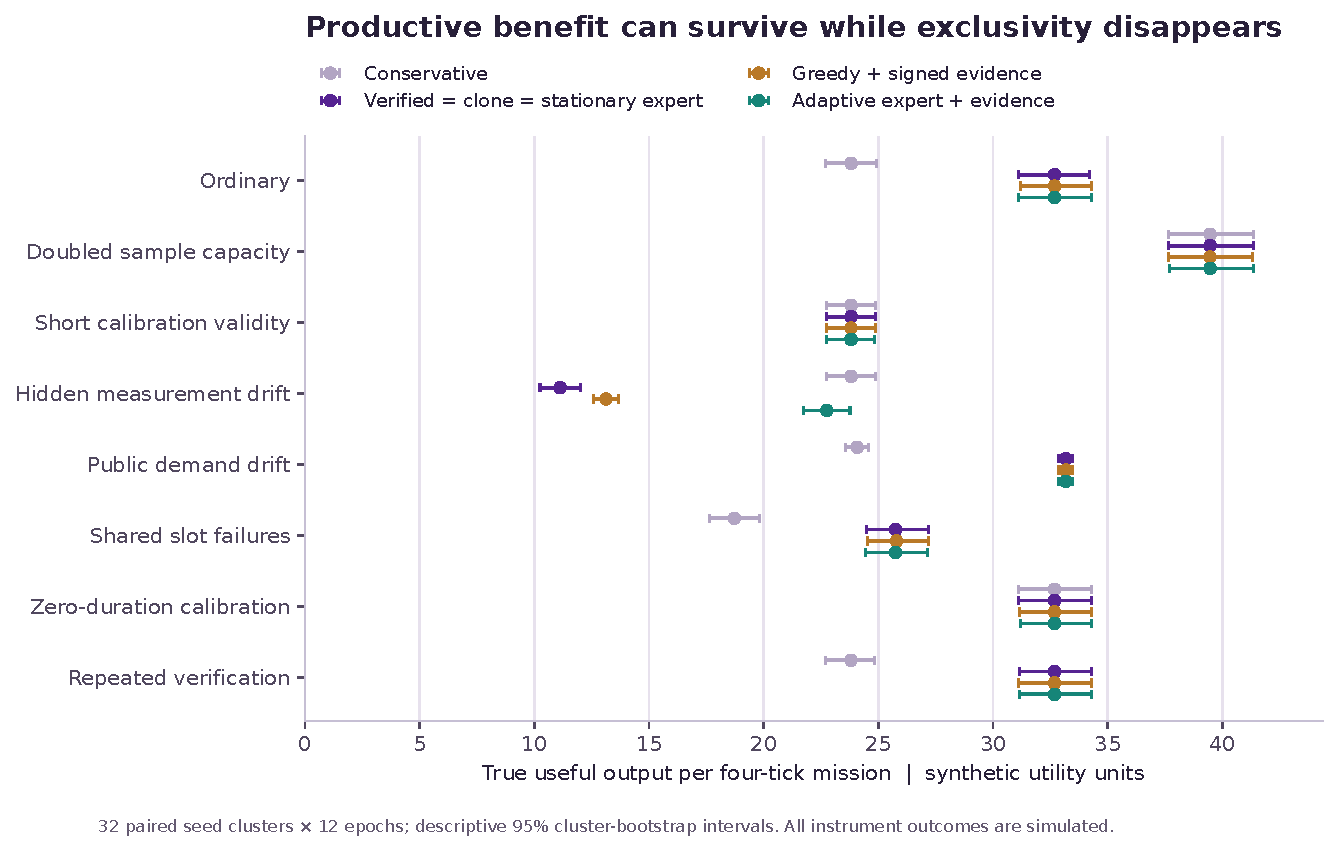
\includegraphics[width=\textwidth]{../figures/condition-outcomes.pdf}
\caption{Measured software outcomes in synthetic worlds. Each point averages 32 seed clusters of 12 epochs; intervals are descriptive cluster-bootstrap intervals. Native verified, complete clone and stationary exact-expert outputs coincide. A positive difference from the conservative restriction does not establish superiority to conventional shared-calibration scheduling.}
\end{figure}

\subsection{Drift reveals what the proof did not establish}
\DriftResults

\begin{figure}[H]\centering
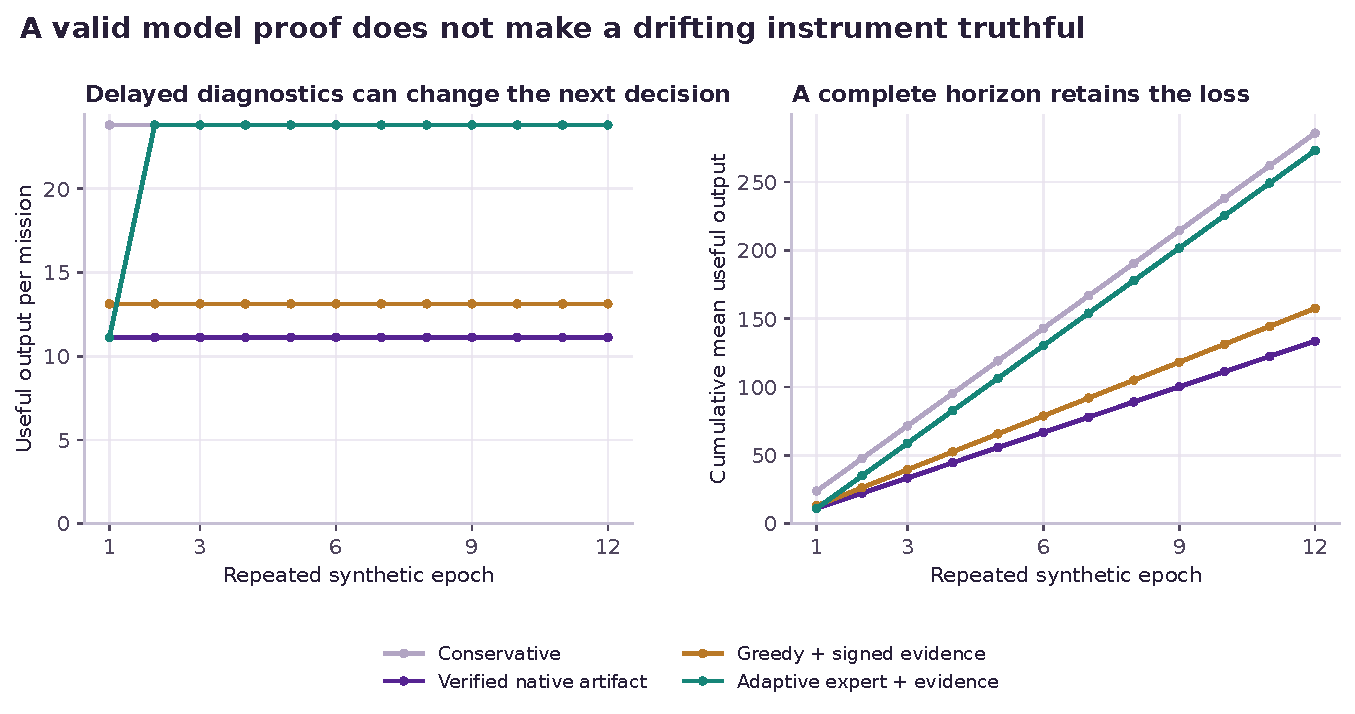
\includegraphics[width=\textwidth]{../figures/drift-and-time.pdf}
\caption{All twelve repeated epochs are shown. The adaptive competitor can use the previous epoch's perfect delayed diagnostic report; the first epoch cannot. The diagnostic channel consumes separately counted auxiliary acquisitions. These are short synthetic missions, not observations of commercial duration or physical calibration reliability.}
\end{figure}

\subsection{The sufficient comparator can be cheaper}
\ComputeResults
The experiment does not award the artifact a benefit simply for carrying more machinery. The independent expert can rebuild the finite allocation and verify its outputs; the simple greedy scheduler is a useful substitute when its assumptions fit. Native proof export may serve an integration or audit purpose, but an unmeasured purpose cannot be booked as an observed gain.

\begin{figure}[H]\centering
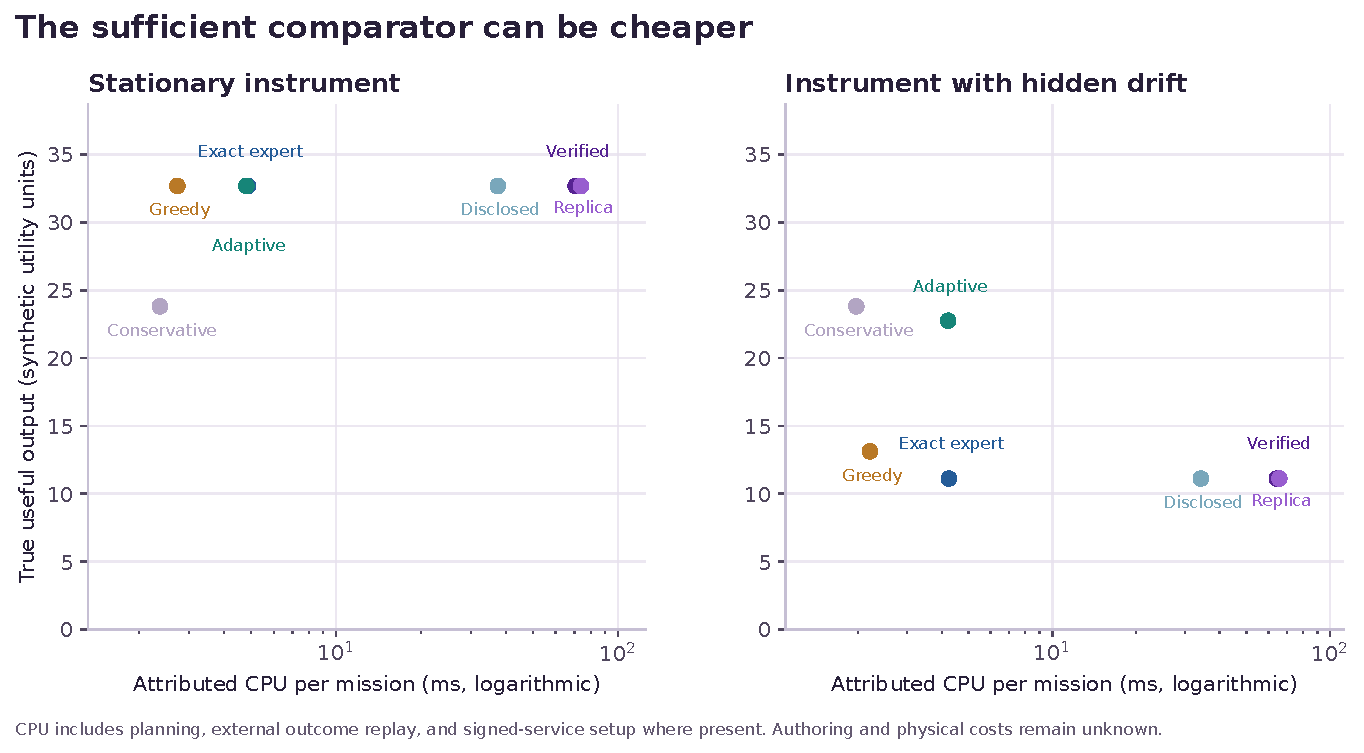
\includegraphics[width=\textwidth]{../figures/output-compute.pdf}
\caption{Output versus measured attributed CPU per mission, including the common external evaluator and the signed-service setup where present. Native optimizer/proof work is separately itemized. The cheaper adequate comparators are retained. Costs omit unknown authoring labor, actual instrument cost and commercial integration.}
\end{figure}

\section{What receipts, registries and contracts establish}
\subsection{Adversarial evidence and the physical-truth boundary}
A receipt can bind an authorized recorder, a mission, source, a plan and an outcome digest. Verification checks those predicates. It cannot establish that a physical sensor produced the claimed observation. The signed-registry controls reject modified payloads, cross-mission replay, expiry, a wrong purpose, an unknown signer, revocation and a changed historical ledger entry. A deliberately false claim signed by the trusted local recorder passes signature verification. This is an expected and necessary negative control.

The finite completion inspector checks the supplied model's allocation and objective. The independent outcome evaluator checks synthetic truth. In the drift condition, these two checks can disagree about usefulness without a software-integrity defect. An attacker who can supply a coherent false world and regenerate its proofs has crossed the study's trusted-input boundary. We do not claim trusted hardware, remote attestation, an independently calibrated sensor, or an external witness.

\subsection{The no-NFT counterfactual}
The local-EVM demonstration binds a compact summary of the actual completed development pilot: six worlds and 42 method records, including the exact raw-data digest. It is a separate mechanism control, not an on-chain execution of the 3,072-world confirmation. The off-chain registry binds the same evidence bytes, plan and base-seed parent commitment and checks once-only routing. Both preserve the same productive result because neither changes the instrument allocator or its physical-model execution. This equality is structurally expected: it tests replacement of the studied evidence-binding interface, not market coordination or every institutional benefit of a public registry.

The local lifecycle executes 113 transactions, including deployment, fixture setup and negative cases. Total simulated gas is 20,701,896; the separately tracked lifecycle subset uses 4,546,309 gas. These are local EVM quantities, not a gas-price quote or a live financial bill. The off-chain record occupies 3,619 bytes. Its construction and repeated verification timings are retained with the source-bound run. These resources cannot be subtracted from one another as though they were a common cost unit.

An off-chain signature requires an independently trusted public key and retained state. The demonstration rejects tampering and an omitted middle record. It also accepts a valid truncated prefix when the verifier has no separately pinned terminal checkpoint. A locally operated EVM can likewise be reset or presented as a different history; this experiment does not confer public-network consensus. Actual public anchoring could provide shared ordering and enforce escrow under additional assumptions. The off-chain control does not replicate decentralized escrow, token custody or public finality.

\scope{\textbf{Registry result.} The NFT layer contributes no measured instrument-output gain in the functional counterfactual. The signed registry is a credible simpler design for the studied evidence-binding service. This does not establish equivalence for every contract function or prove that on-chain accountability has no institutional value.}

\subsection{Open knowledge and limited disclosure}
The open branch publishes algorithms, source, reproduction instructions and synthetic inputs. The restricted branch uses Node/OpenSSL AES-256-GCM with a fresh ephemeral 256-bit key, a fresh 96-bit nonce and mission-associated authenticated data \citep{dworkin2007}. Both voluntarily authorized operators receive the same plaintext; outsider access is restricted. Authorized decryption, wrong-key rejection, changed ciphertext rejection and changed-mission rejection are tested. No encryption key is persisted. Metadata and length remain visible. Since the generator and final synthetic workloads are public, this demonstrates disclosure-control functionality, not secrecy of the published experiment.

A small-domain commitment test recovers an unsalted SHA-256 calibration label by enumerating 16 possibilities. Hashes are commitments, not encryption. Withholding a key is an access restriction and is never counted as superior productive capability. Ed25519 is the existing signature primitive, not new cryptography \citep{rfc8032}.

\subsection{Five contracts, verified source semantics}
All five requested contracts are byte-identical between \href{https://github.com/MontrealAI/AGI-Alpha-Agent-v0/tree/197147ffd22c5ae13113162afffaf3ce9c10aa2e/contracts/ascension}{observed Alpha source \code{197147ff...}} and the full historical reference \code{c0fc5217e364a39a4cd123d17a8317c06b80f820}. This is a source comparison, not a fresh verification of live bytecode or activation. The complete source hashes, exact line links, compiler policy and local outputs appear in the companion audit.

\textbf{NovaSeed.} The ERC-721 stores capsule, plan and evidence commitments, a creator, a parent and a job count. Commitments must be nonzero; the job bound is 1--128; the metadata URI has a bounded length. A nonzero parent must be owned by the caller. A commitment does not encrypt its contents, validate a plan's productive merit, guarantee availability, or confer intellectual-property rights.

\textbf{AscensionAccess and AscensionRiskOracle.} Access checks current ENS ownership and bounded governance admission. Risk review uses eligible staked validators, a configured quorum and time-limited approval. Parent approval is not successor approval. Address separation is not proof of beneficial or institutional independence. Admission restrictions are permissions, not measurements of ability.

\textbf{AscensionMark.} An eligible seed owner opens a funding campaign with bounded target and timing. Funding lots provide internal accounting; they are not equity or a dividend promise. Funding-lot purchases and transfers have phase/time restrictions. Unused lot sales retain a withdrawal path while the phase is Funding, including after its funding deadline. Bloom requires the Funding phase, sufficient reserve, current owner/admission/risk conditions and a timestamp strictly before \code{fundingEnd}. It changes phase to Bloomed, sets the execution end and emits an event. Bloom neither burns the NFT nor mints a new agent, generates profit or locks general token circulation.

The Merkle plan commits the job index and specification. Routing checks membership, bounds and the unused index; the once-only flag is set before the external job post. The stored JobMarket specification hash uses index zero, while the Mark route event preserves the indexed plan leaf. These are distinct hashes for later indices. Unused or returned reserves can be reclaimed according to closure and pro-rata accounting; executed expenditure does not guarantee principal recovery.

\textbf{AscensionJobMarket.} The code implements opted-in staked roles, per-bid collateral, three selected reviewers and exact submitted-artifact hashes. Two approving votes can settle the job; failure, refund and collateral consequences follow their specified paths. The gross review pool is 5\%, and each actual payout burns its integer-floor 1\% share. That payout mechanism is separate from Bloom. Local execution exercises these semantics with mock assets, never live funding or trade. The Manager USDC route remains a different denomination and accounting path.

\section{Economics with separate accounts}
\subsection{A cost vector before a currency claim}
For each policy we retain attempted samples, useful samples, failures, calibration acquisitions, auxiliary diagnostic acquisitions, occupied instrument ticks, measured CPU and wall time, model/proof bytes, signed-record bytes and verification work. A failed measurement consumes its sample and instrument time. Candidate enumeration is computation, not an instrument acquisition. Four auxiliary diagnostic acquisitions per epoch are reported separately from the contested four-tick instrument horizon.

The recorded campaign totals include parent and worker CPU, source copying, worker startup, evidence construction and stored bytes. The parent entry-point imports before the campaign timer and the final metrics serialization are outside that timer. Method comparisons additionally identify compiler/solver, inspection, external evaluator and recorder-setup components. Common measured harness overhead is retained. Construction labor, AI-assisted authoring cost, opportunity cost, real instrument depreciation, physical energy and willingness to pay were not fully metered. No result is therefore called full-cost commercial profitability.

\CostTable

\AdditionalCosts

Let $u$ be an assumed monetary value per useful synthetic utility unit, $p_c,p_s,p_d$ assumed prices per calibration, sample and auxiliary diagnostic acquisition, and $p_{\rm cpu}$ an assumed CPU-hour price. For two alternatives, the illustrative difference is
\begin{equation}
\Delta W=u\Delta U-p_c\Delta n_c-p_s\Delta n_s-p_d\Delta n_d
-\frac{p_{\rm cpu}}{3600}\Delta t_{\rm cpu}-\Delta H,
\end{equation}
where $\Delta H$ includes unmeasured human and other omitted costs. This is a sensitivity equation, not a measured cash account. If $\Delta U>0$, its break-even value is the remaining cost difference divided by $\Delta U$. If two fully equipped methods have equal $U$, positive additional cost cannot be justified by that output metric alone. Additional audit or institutional benefits would need separate measurement.

The ordinary capability replaces a calibration tick with a sample tick. It can therefore increase useful output while reducing calibration acquisitions and increasing sample acquisitions. It does not demonstrate that all kinds of physical cost fall. In the zero-duration-calibration condition, the restrictive baseline can catch up without the artifact's operational change. In short-validity conditions, shared calibration cannot simply be extended by software. These stress conditions are tests of the asserted bottleneck.

\SensitivityResults

\subsection{Capture is conditional on a market that was not observed}
Suppose a producer charges $p$ for accepted service. Then $R=pq$ is modeled revenue and $R-C$ is modeled profit. Actual customer revenue in this study is zero. No buyer commitment, paid pilot, intellectual-property exclusivity, rights dispute or instrument lease was observed. The two native currency routes use zero caps and no financial execution; local mock-token settlements are not proceeds.

A homogeneous-service price-competition scenario with identical complete replicas, equivalent access, sufficient capacity and no switching cost permits the innovation-specific premium to vanish. That is a conditional economic interpretation of measured service equality, not a theorem that all inventor profits must vanish. Scarce capacity, distribution, service quality, liability, legitimate rights or a better deployed capability could alter capture. None is automatically exclusive or enduring. We do not infer such an asset from an NFT, an admission whitelist, a token balance, an intelligence claim or a repository's existence.

Copying and process-startup timings quantify a warm-host software operation. They omit acquiring the host, installing Node, understanding the system, hiring an operator and arranging legitimate physical access. Independent expert authoring time was not metered. Consequently, we do not convert a subsecond source operation into a forecast of market catch-up time. The finite horizon demonstrates repeated service outcomes; it does not measure a commercial moat over months or years.

\scope{\textbf{Economic conclusion.} A positive operational benefit against redundant recalibration can coexist with zero residual output advantage against a complete copy and higher computing cost than a sufficient conventional implementation. The shared capability may be valuable even when the observed test gives the inventor no basis for an exclusive premium. Real social surplus and private profit remain unmeasured.}

\clearpage
\section{Integration, limitations and interpretation}
\subsection{Actual reuse and current boundaries}
\begin{table}[H]\small\renewcommand{\arraystretch}{1.15}
\begin{tabularx}{\textwidth}{@{}>{\raggedright\arraybackslash}p{0.24\textwidth}>{\raggedright\arraybackslash}p{0.23\textwidth}>{\raggedright\arraybackslash}X@{}}\toprule
Foundation & Status & Evidence and limit\\\midrule
Alpha finite optimizer/inspector & Executed on new workload & Exact vendored import closure; finite calibration model, assignment, completion inspection and declared work ledger.\\
Jobs signatures & Executed on new workload & Existing purpose/context-bound Ed25519 signing and verification; ephemeral fixture keys.\\
Fleet outcome ledger & Executed on new workload & Existing hash-chain append/reopen/check; unknown monetary costs preserved. No external Fleet worker provisioned.\\
Published JobDispatcher & Executed local lifecycle & Real pure callbacks, typed world/policy declarations and fresh evidence in two mission graphs. Not the separately held Harness branch.\\
Manager USDC route & Executed supported native mission & Six native stages plus a stronger successor checked; insufficient budget inconclusive; invalid measurement rejected; zero cap, no authority.\\
Jobs AGIALPHA route & Executed same native mission & Same frozen workspace and evidence scope; separate denomination, no conversion or financial execution.\\
New workload native commissioning & Unavailable/unqualified & The native Discovery Lab schema does not automatically admit this instrument workload.\\
Five Ascension contracts & Executed local EVM & Exact source, mock ENS/assets, lifecycle and failure controls; no live financial action or production readiness.\\\bottomrule
\end{tabularx}
\caption{Source-read, executed and unavailable paths are different statuses. No missing adapter is replaced by an invented API.}
\end{table}

The Manager and Jobs native tests intentionally retain the Alpha revision required by their installed harnesses, \code{0385df4c...}, while the new optimizer uses observed Alpha source \code{197147ff...}. They share a frozen native workspace digest, not a claim that every current repository revision is mutually installed and qualified. Both preserve accepted, rejected, inconclusive and renewed histories. The result is eighteen receiver observations, including four negative/inconclusive cases; these are not eighteen independent instrument experiments.

The published dispatcher implements seven job families: constitution, evidence, formation, challenge, verification, admission and renewal. They are not renamed as the seven TI labels. Our thin wrapper relates real bounded work to the intended journey: Identify fixes the mission; Out-Learn consumes declared calibration and development evidence; Out-Think constructs the finite world model; Out-Design packages its executable capability; Out-Strategise selects a plan; Out-Execute replays its actual synthetic observations; Out-Evolve compares a fresh successor/copy under new scope. The local graph performs actual enumeration, replay, input binding and evidence checks. Its prior Node execution is explicitly precomputed evidence, not a subprocess secretly launched inside the dispatcher.

\LifecycleResults

World, Policy, Proof and Authority remain separate. The world describes predictions and possible failures; the policy chooses work; the proof checks a specified statement against specified evidence; authority is current permission for a bounded action. Inherited governance does not supply an unseen successor's permission or competence. Distinct local role identities improve attribution but do not create external organizational independence. The signed reports grant no production authority.

\subsection{Limits that materially change the interpretation}
First, the physical resource is simulated. Four jobs and four ticks make an exact independent check feasible, but they do not establish scalability, complex scientific validity or real laboratory throughput. Integer weights are supplied priorities, not empirical willingness to pay. The base case is simple enough for a conventional greedy policy to tie the more elaborate system; that is a useful limitation of the claimed contribution.

Second, the reported independent expert is independent code within the same assisted study. It is not an external professional team or a measured human reconstruction exercise. A complete clone is an existence witness for copying, not independent discovery. Warm-host startup excludes environment procurement and comprehension.

Third, delayed diagnostics are ideal, explicit and costly in their own resource class. Adaptive recovery depends on a repeatable within-batch drift profile and correct retrospective observations. No claim is made about an adversarial or rapidly changing instrument that defeats that extrapolation. A source-bound proof of a model cannot repair a wrong world model by itself.

Fourth, service records are controlled local fixtures. No trusted-hardware attestation, independent sensor provenance, multi-party custody, public consensus finality, or third-party acceptance is demonstrated. The signed falsehood and truncated-log controls expose those limits directly.

Fifth, source and local execution qualify only the named paths. New-domain native commissioning, installed four-repository delivery, held Harness/Fleet operations and richer-site qualification remain separate work. Passive publication must follow the existing coordinator's receipt, catalogue and review path. A public file or a passing local test does not clear an unrelated hold.

Finally, this is not a test of AGI, ASI, market prediction, a permanent moat, unlimited wealth or token appreciation. \TI\ is used as a research discipline: identify a restriction, construct an enabling alternative, test it against strong replacements, preserve scope and let unfavorable evidence change the conclusion.

\subsection{Interpretation}
The useful object is a transferable capability and its inspectable evidence. Its value need not depend on secrecy or enforced exclusivity. The complete copying test asks whether another equipped operator can obtain the same productive result; the strongest comparator asks whether it can do better or do enough more cheaply. The tested outcomes decide those questions within the declared model. The result may be public abundance rather than an inventor's exclusive advantage, and that is a successful scientific distinction rather than a failed narrative.


\clearpage
\appendix
\section{Reproduction and evidence map}
\subsection{Three levels of reproduction}
The full source archive includes this canonical compiled PDF, monolithic and structured LaTeX, bibliography, vector figure sources, executable modules, pinned upstream dependencies and licenses, raw compressed records, analysis, negative controls, source audits and a SHA-256 manifest. The source ZIP is reopened and every member checked before delivery. The original compiled PDF digest is retained inside it; a later download wrapper is not substituted for that canonical byte sequence.

\textbf{Quick experiment.} Enter the archive's \code{research/} directory. With Node 24 available, run \code{node src/run\_experiment.mjs --mode pilot --out results/my-pilot}. This runs six worlds and seven methods, creates a fresh copied worker and separate signed evidence, and retains failures. The output directory must be new; originals are never overwritten.

\textbf{Replay the published evidence.} Run \code{node audit/verify\_results.mjs results/holdout-01}. It recomputes outcomes, checks the public signatures, mission bindings, delayed diagnostic equality and actual ledger chains. The retained native completion files can be inspected with the unchanged Alpha checker. The archive's manifest independently detects byte changes. Historical fixture verification grants no present permission.

\textbf{Repeat the entire confirmation.} From \code{research/}, run:
\begin{quote}\small\ttfamily
node src/run\_experiment.mjs --mode holdout --out results/my-holdout\\
python analysis/analyze.py results/my-holdout
\end{quote}
The runner requires the frozen source inventory. Node 24.19.0 was used for the recorded campaign. The Python analysis uses NumPy; plotting additionally uses Matplotlib. Resource limits and model assumptions are part of the protocol. Random mission IDs, ephemeral keys, timestamps, timing and resulting signatures will differ; deterministic workload outcomes and exact comparison predicates should agree.

The local EVM is a separate optional reproduction: install the hash-pinned npm lockfile in the provided contract test directory, compile using the retained Solidity 0.8.37 profile, and execute the bounded local script. The guide records the via-IR optimizer policy and the exact historical source comparison. No live RPC, key, token purchase or wallet action is required or permitted by the demonstration.

The archive's root guide also links the actual published dispatcher bridge and both native routes. The dispatcher uses fresh output filenames under \code{contracts-audit/lifecycle/}. Native route reconstruction uses \code{foundations/reproduce-routes.py}, Git and network access to the exact public revisions; it does not commission the new instrument workload. Recorded environments and dependency locks accompany each lane.

To rebuild the PDF, enter \code{paper/} and run \code{latexmk -pdf paper.tex}. Figure scripts and generated numerical macros are included. The original canonical PDF is preserved even when a rebuild produces different metadata or font-subset bytes.

\subsection{Exact repository identities}
\begin{table}[H]\footnotesize\renewcommand{\arraystretch}{1.2}
\begin{tabular}{@{}ll@{}}\toprule
Repository & Inspected revision\\\midrule
AGI-Alpha-Agent-v0 & \texttt{197147ffd22c5ae13113162afffaf3ce9c10aa2e}\\
AGIJobManager & \texttt{c5958eae872458c2f3cac48fea0b4bbfadc6ac6c}\\
AGIJobsv0 & \texttt{9983478d42c32fe399f28dd9b0e0173f904b8a11}\\
AGI-Fleet-Linux & \texttt{45759fb096faf8988f58ae5ea71248d0f35a97c7}\\
Native route's selected Alpha & \texttt{0385df4c9728db19c396e039cd04678eebfddb9e}\\
Historical five-contract comparison & \texttt{c0fc5217e364a39a4cd123d17a8317c06b80f820}\\\bottomrule
\end{tabular}
\caption{Immutable source snapshots, not assertions that moving main branches remain at these commits.}
\end{table}

The three foundation PDFs were read at the inspected Alpha revision: \href{https://github.com/MontrealAI/AGI-Alpha-Agent-v0/blob/197147ffd22c5ae13113162afffaf3ce9c10aa2e/docs/Transformational_Intelligence.pdf}{Transformational Intelligence}, \href{https://github.com/MontrealAI/AGI-Alpha-Agent-v0/blob/197147ffd22c5ae13113162afffaf3ce9c10aa2e/docs/Invent_the_Economy.pdf}{Invent the Economy}, and \href{https://github.com/MontrealAI/AGI-Alpha-Agent-v0/blob/197147ffd22c5ae13113162afffaf3ce9c10aa2e/docs/papers/possibility-foundry-v1.pdf}{The Possibility Foundry, v1}. Their exact digests are in the archive's \code{foundations/evidence/source-pins.json}. The recovered Foundry's actual path includes \code{docs/papers/}.

\subsection{Contract source map}
All links below pin the same inspected Alpha revision. Line ranges identify the implementation read, not a semantic guarantee about future revisions.

\begin{itemize}
\item \href{https://github.com/MontrealAI/AGI-Alpha-Agent-v0/blob/197147ffd22c5ae13113162afffaf3ce9c10aa2e/contracts/ascension/NovaSeed.sol\#L7-L37}{NovaSeed, lines 7--37}: ERC-721 commitments, parent and bounded jobs/URI.
\item \href{https://github.com/MontrealAI/AGI-Alpha-Agent-v0/blob/197147ffd22c5ae13113162afffaf3ce9c10aa2e/contracts/ascension/AscensionAccess.sol\#L24-L77}{AscensionAccess, lines 24--77}: current ENS ownership and expiring admission.
\item \href{https://github.com/MontrealAI/AGI-Alpha-Agent-v0/blob/197147ffd22c5ae13113162afffaf3ce9c10aa2e/contracts/ascension/AscensionRiskOracle.sol\#L39-L112}{AscensionRiskOracle, lines 39--112}: stake, review round, quorum, owner/creator exclusion and current approval.
\item \href{https://github.com/MontrealAI/AGI-Alpha-Agent-v0/blob/197147ffd22c5ae13113162afffaf3ce9c10aa2e/contracts/ascension/AscensionMark.sol\#L52-L146}{AscensionMark, lines 52--146}: funding lots, Bloom, once-only indexed routing, closure and reserve reclaim.
\item \href{https://github.com/MontrealAI/AGI-Alpha-Agent-v0/blob/197147ffd22c5ae13113162afffaf3ce9c10aa2e/contracts/ascension/AscensionJobMarket.sol\#L92-L242}{AscensionJobMarket, lines 92--242}: plan hashing, roles, collateral, artifact-bound votes, payouts, refunds and reputation.
\end{itemize}

\subsection{Claim--evidence--cost ledger}
\ClaimLedger

\textbf{Reproducibility identity.} \FreezeIdentity

\textbf{Publication custody.} Coordination uses \href{https://github.com/MontrealAI/AGI-Alpha-Agent-v0/issues/4850}{issue \#4850}. The receiving boundary in comment \href{https://github.com/MontrealAI/AGI-Alpha-Agent-v0/issues/4850\#issuecomment-6377105309}{6377105309} reserves shared catalogue, merge and Pages publication for the existing coordinator. Original runtime holds remain separate. The companion's publication record states the actual source PR, checks and served-byte status; this manuscript does not turn an uncompleted deployment into a finding.

\textbf{Authoring and review.} This edition was prepared with AI-assisted research, coding, literature inspection and delegated same-session adversarial review. Separate implementations and source checks are reported precisely; they do not imply external peer review. Human authoring time and attributable model costs were not completely metered. No sensitive data, private credentials, real asset transfer or paid infrastructure was used by the local study.


\clearpage
\bibliographystyle{plainnat}
\bibliography{bibliography}
\end{document}
